\documentclass[thesis.tex]{subfile}

\chapter{Space-tiling and the Devito compilation process}
\label{ch:devito}

% TODO: elaborate
This chapter provides a summary of the existing Devito compilation process, in particular the existing implementation of spatial-tiling (Section~\ref{sec:spatial-tiling}).


\section{The Devito symbolic engine (DSE)}
\label{sec:dse}

The Devito symbolic engine is responsible for stencil optimisation and common sub-expression elimination (CSE).
At this point the indices and loops have not been generated yet.
Although we are working with loop transformations, we chose to perform skewing (Section~\ref{sec:skewing}) here, as skewing is a modification on the canonical indexing scheme.

% TODO: examples


\section{The Devito loop engine (DLE)}
\label{sec:dle}

The DLE performs loop transformations including loop fission and tiling, while also marking loops to be executed in parallel or that denormal numbers should be flushed.
Before it is invoked, the loops are built from the previously-manipulated expressions; clearly it would not be possible to implement tiling before this stage.



\section{Spatial tiling in Devito}
\label{sec:spatial-tiling}

Under the existing tiling transformation, tiling is performed over every dimension but the innermost, which benefits from vectorisation.
In the generated stencils, skewing is not required, as dependencies do not cross tile boundaries, instead referencing values computed in the previous time iteration.

\subsection{Remainder loops}
When discussing loop tiling in Section~\ref{sec:bg-loop-tiling}, we constrained our tiles with \texttt{min} constraints.
To deal with the case when the tile size does not divide the extent of the iteration space, Devito instead implements \emph{remainder loops}, which Figures~\ref{fig:tiled-remainder-space} and~\ref{lst:remainder} illustrate.

\begin{figure}[!ht]
	\centering
	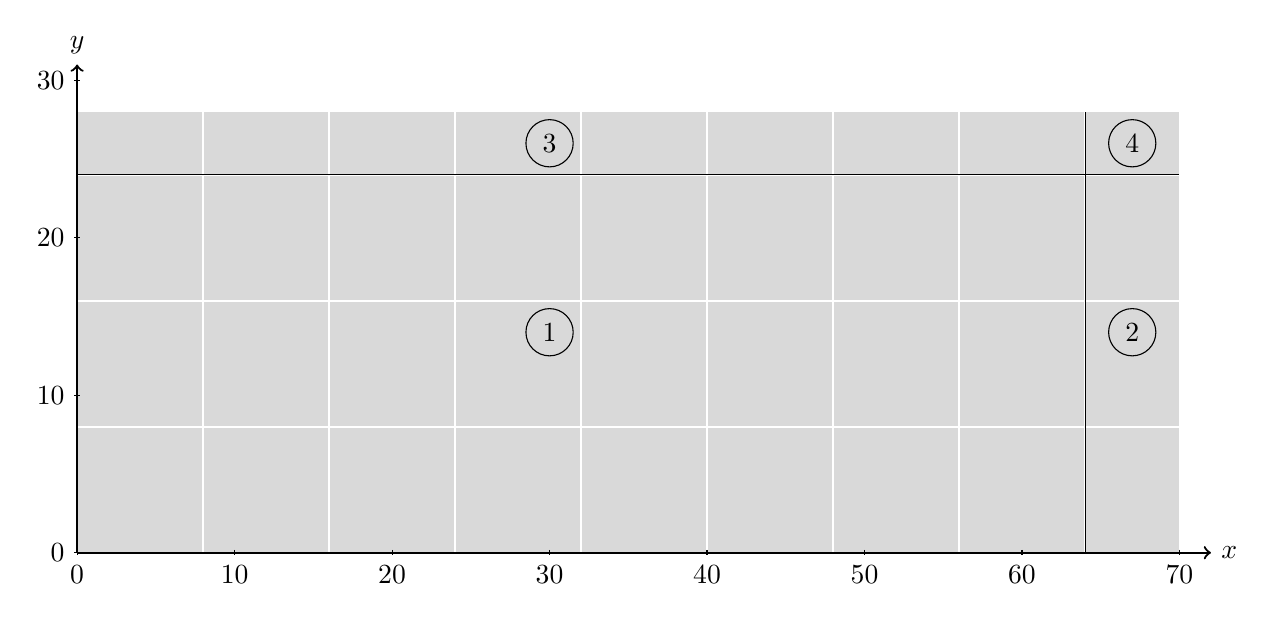
\begin{tikzpicture}
	\fill[gray!30!white] (0,0) rectangle (14,5.6);
	\draw[step=1.6cm,white,thick] (0,0) grid (14,5.6);
	
	\draw[thick,->] (0,0) -- (14.4,0) node[right]{$x$};
	\draw[thick,->] (0,0) -- (0,6.2) node[above]{$y$};
	
	\foreach \x in {0,10,20,30,40,50,60,70}
	\draw (\x*0.2 cm,1pt) -- (\x*0.2 cm,-1pt) node[anchor=north] {$\x$};
	\foreach \y in {0,10,20,30}
	\draw (1pt,\y*0.2 cm) -- (-1pt,\y*0.2 cm) node[anchor=east] {$\y$};
	
	\draw[xstep=12.8,ystep=4.8,black,very thin] (0,0) grid (14,5.6);
	\draw (6,2.8) circle [radius=0.3] node {$1$};
	\draw (13.4,2.8) circle [radius=0.3] node {$2$};
	\draw (6,5.2) circle [radius=0.3] node {$3$};
	\draw (13.4,5.2) circle [radius=0.3] node {$4$};
	\end{tikzpicture}
	\caption{Tiles over an iteration space. Note that the tile size need not be the same in each dimension, or divide the extent of the iteration cleanly.}
	\label{fig:tiled-remainder-space}
\end{figure}

\begin{figure}[!ht]
\begin{lstlisting}
for (int x_blk = x_s; x_blk < x_e - (x_e-x_s)%x_bs; x_blk += x_bs)
  for (int y_blk = y_s; y_blk < y_e - (y_e-y_s)%y_bs; y_blk += y_bs)
    for (int x = x_blk; x < x_blk + x_bs; x++)
      for (int y = y_blk; y < y_blk + y_bs; y++)
        A[x][y] = B[x][y] + B[x][y+1];  // Nest 1

for (int x = x_e - (x_e-x_s)%x_bs; x < x_e; x++)
  for (int y_blk = y_s; y_blk < y_e - (y_e-y_s)%y_bs; y_blk += y_bs)
    A[x][y] = B[x][y] + B[x][y+1];  // Nest 2

for (int x_blk = x_s; x_blk < x_e - (x_e-x_s)%x_bs; x_blk += x_bs)
  for (int y = y_e - (y_e-y_s)%y_bs; y < y_e; y++)
    A[x][y] = B[x][y] + B[x][y+1];  // Nest 3

for (int x = x_e - (x_e-x_s)%x_bs; x < x_e; x++)
  for (int y = y_e - (y_e-y_s)%y_bs; y < y_e; y++)
    A[x][y] = B[x][y] + B[x][y+1];  // Nest 4
\end{lstlisting}
	\caption{Replacement of \texttt{min} constraints with remainder loops from Figure~\ref{lst:interchange}. First the main tiles, then the remainder in \texttt{x} then \texttt{y} dimensions, and finally the remainders in both dimensions. Braces removed for concision.}
	\label{lst:remainder}
\end{figure}